\documentclass[a4paper,12pt]{article} %style de document
\usepackage[utf8]{inputenc} %encodage des caractères
\usepackage[french]{babel} %paquet de langue français
\usepackage[T1]{fontenc} %encodage de la police
\usepackage[top=2cm,bottom=2cm,left=2cm,right=2cm]{geometry} %marges
\usepackage{graphicx} %affichage des images
\usepackage{amssymb}
\usepackage{url}
\usepackage{verbatim}
\usepackage{amsmath}
\usepackage{color}
\usepackage{tikz}
\usepackage{hyperref}
\hypersetup{
	hidelinks,
    colorlinks,
    citecolor=black,
    filecolor=black,
    linkcolor=black,
    urlcolor=black
}

\begin{document} %début du document

%----------------------------------
%page de garde
%----------------------------------

\begin{titlepage}

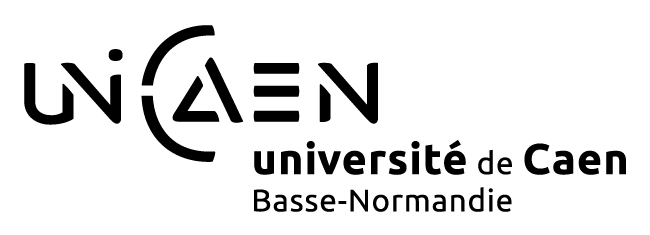
\includegraphics[scale=0.3]{images/unicaen.png}

\vspace{7cm}

\begin{center}

\begin{Huge}
Méthodes de conception\\
Rapport de Projet\\
\end{Huge}
\vspace{2cm}
\begin{large}
Beauchamp Aymeric 21301016\\
Demé Quentin 21507097\\
Jacqueline Martin 21507982\\
Zaizafoun Sami 21600538\\
\vspace{1cm}
L3 Informatique  Groupe A2
\end{large}

\end{center}
\end{titlepage}


%------------------------------
%sommaire
%------------------------------

\newpage

\tableofcontents

\newpage

%------------------------------
%contenu
%------------------------------

\section*{Présentation du projet}

L'application à développer est un jeu de stratégie au tour par tour. Chaque joueur peut se déplacer sur une grille de jeu et utiliser des armes pour vaincre ses adversaires, le but étant d'être le dernier joueur vivant.\\
Nous avons pris quelques libertés par rapport au sujet de base : chaque joueur dispose ainsi de points de vie et de points d'action, au lieu d'une simple quantité d'énergie.
Les joueurs perdent lorsqu'ils n'ont plus de points de vie, et utilisent les points d'action pendant leur tour pour effectuer leurs actions (se déplacer, tirer, utiliser le bouclier...). Les points d'action sont restitués au début du tour d'un joueur.\\
Pendant un tour, les joueurs peuvent agir autant qu'ils le veulent, tant qu'ils ont assez de points d'action pour le faire. Le tour d'un joueur se termine quand il n'a plus de points d'actions ou quand il décide de passer sans dépenser ce qui lui reste.

\section{Organisation du code}

L'application est séparée en deux packages : le package modele qui contient tout ce qui est nécessaire au fonctionnement du jeu, et le package graphics qui permet l'utilisation du jeu en interface graphique.

\begin{figure}[!h]
\centering
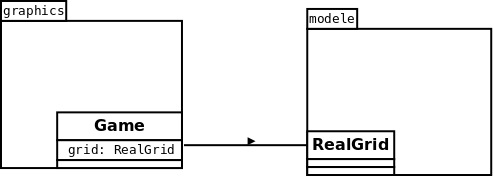
\includegraphics[scale=0.5]{images/packages.png}
\caption{Diagramme de packages}
\end{figure}

\begin{figure}[!h]
\centering
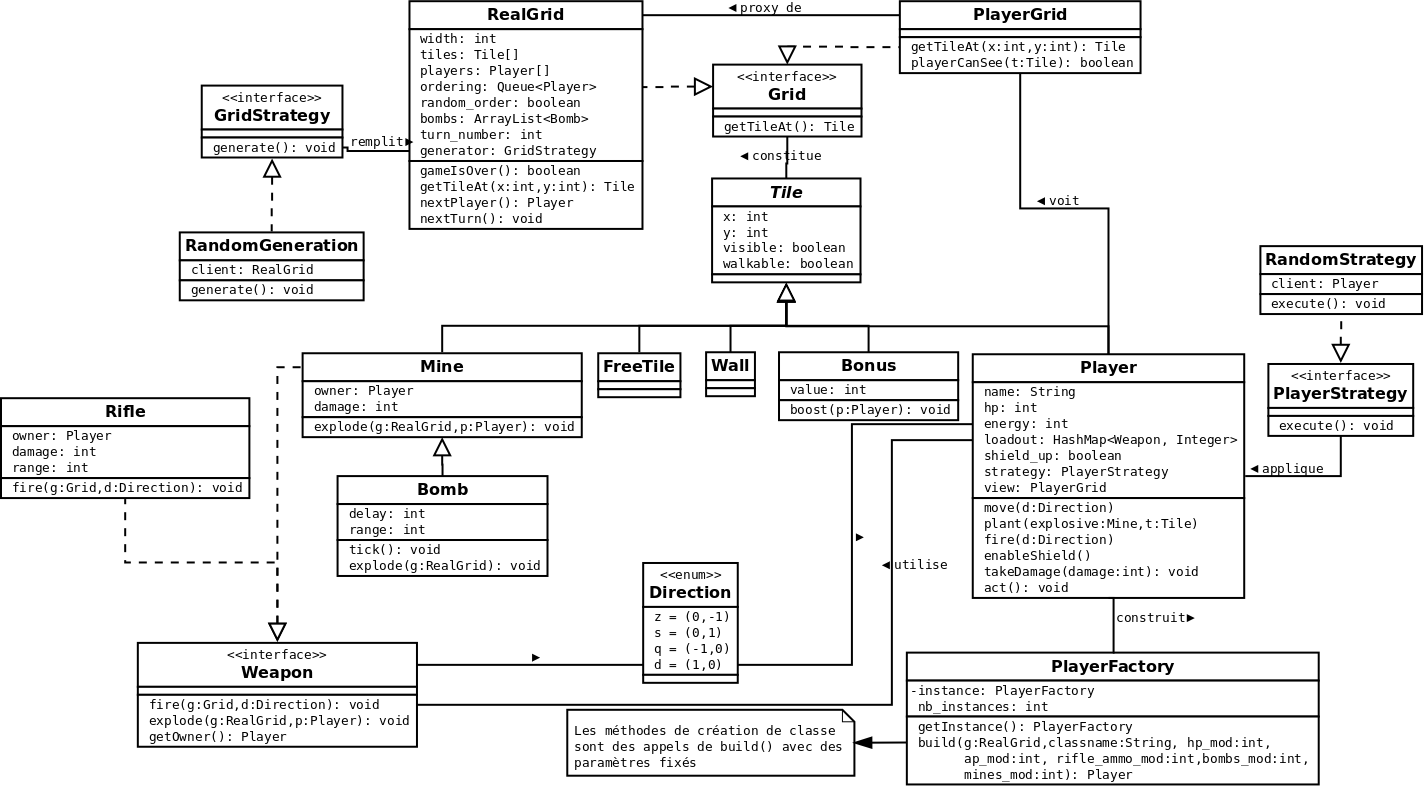
\includegraphics[scale=0.33]{images/modele.png}
\caption{Diagramme de classe du package modele}
\end{figure}


\section{L'interface graphique}
\subsection{La classe ImagesLoader}
La classe ImagesLoader est une classe s’occupant de gérer le chargement des images et de facilité leur utilisation au sein du package \textit{graphics}. Nous allons quelque peu détailler son fonctionnement.
\subsubsection{Découpage du tileset}
Les images sont découpées au sein d'une même image d'ensemble: \textit{le titeset}. Le découpage de ce tileset se fait du coin en haut à gauche, jusqu'au coin inférieur droit. Cette ordre a son importance puisque la position de l'image dans la liste correspond à l'index récupéré dans le XML moins un.
\begin{figure}[!h]
\centering
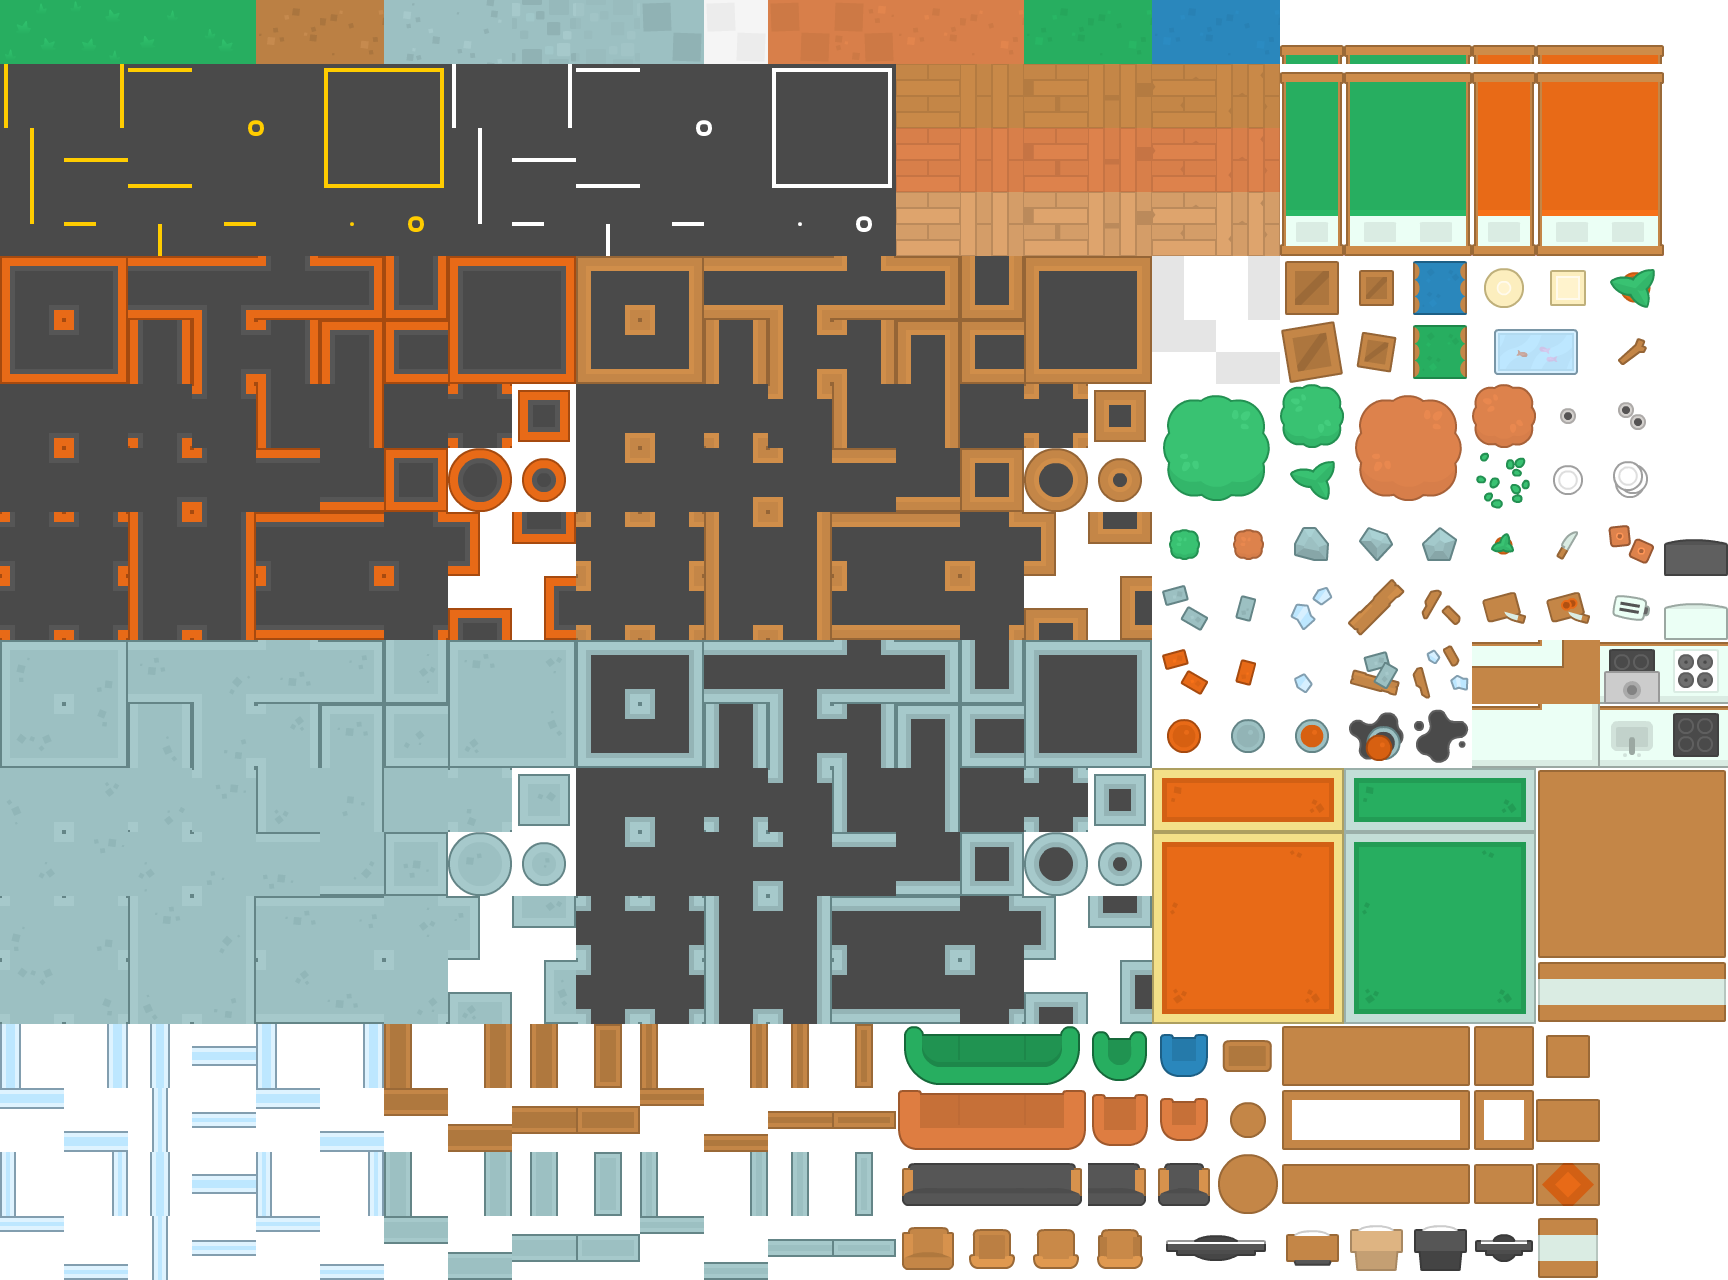
\includegraphics[scale=0.12]{images/tileset.png}
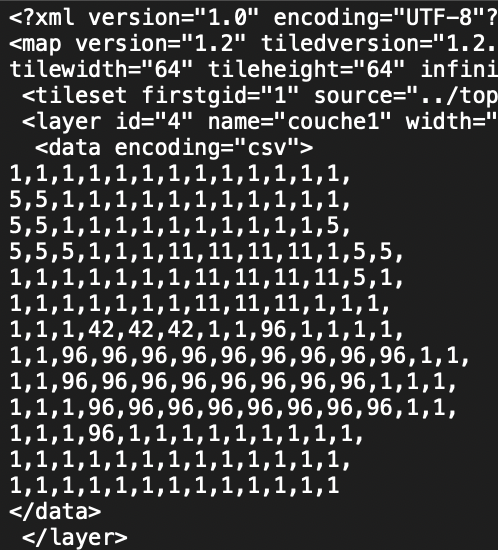
\includegraphics[scale=0.5]{images/XML.png}
\caption{Mise en parallèle du XML et du tileset}
\end{figure}
\newline
Comme on peut le voir sur la figure ci-dessus, les indices 1 correspondent à l'image 0 du tileset qui est l'image en haut à gauche de ce dernier.
\subsubsection{Utilisation}
Cette classe a pour but de charger les images nécessaires à l’affichage du jeu. Ces ressources sont créées comme étant \textit{static} pour être accessible de n’importe où sans passer par des getters. Le chargement des images nécessite tout de même un appel en début de programme de la méthode loadImages().
Ce fichier regroupe les images :
\begin{itemize}
\item Des entités d’environnement du jeu (ArrayList)
\item Des personnages (HashMap<Integer, ArrayList>)
\item Du bouclier
\item Des mines, et des bombes
\item Des bonus
\end{itemize}
Ces images sont utilisées pour créer les objets de classe \textit{Tile}. En effet, un \textit{Tile} est créée avec ses coordonnées \textit{x} et \textit{y} et une image étant sa représentation graphique.
\subsection{La classe View}
La classe view est la classe permettant l’affichage du model en vue graphique. Le code possède également une classe ViewConsole qui réalise un affichage console en permettant de jouer. 

\begin{figure}[!h]
\centering
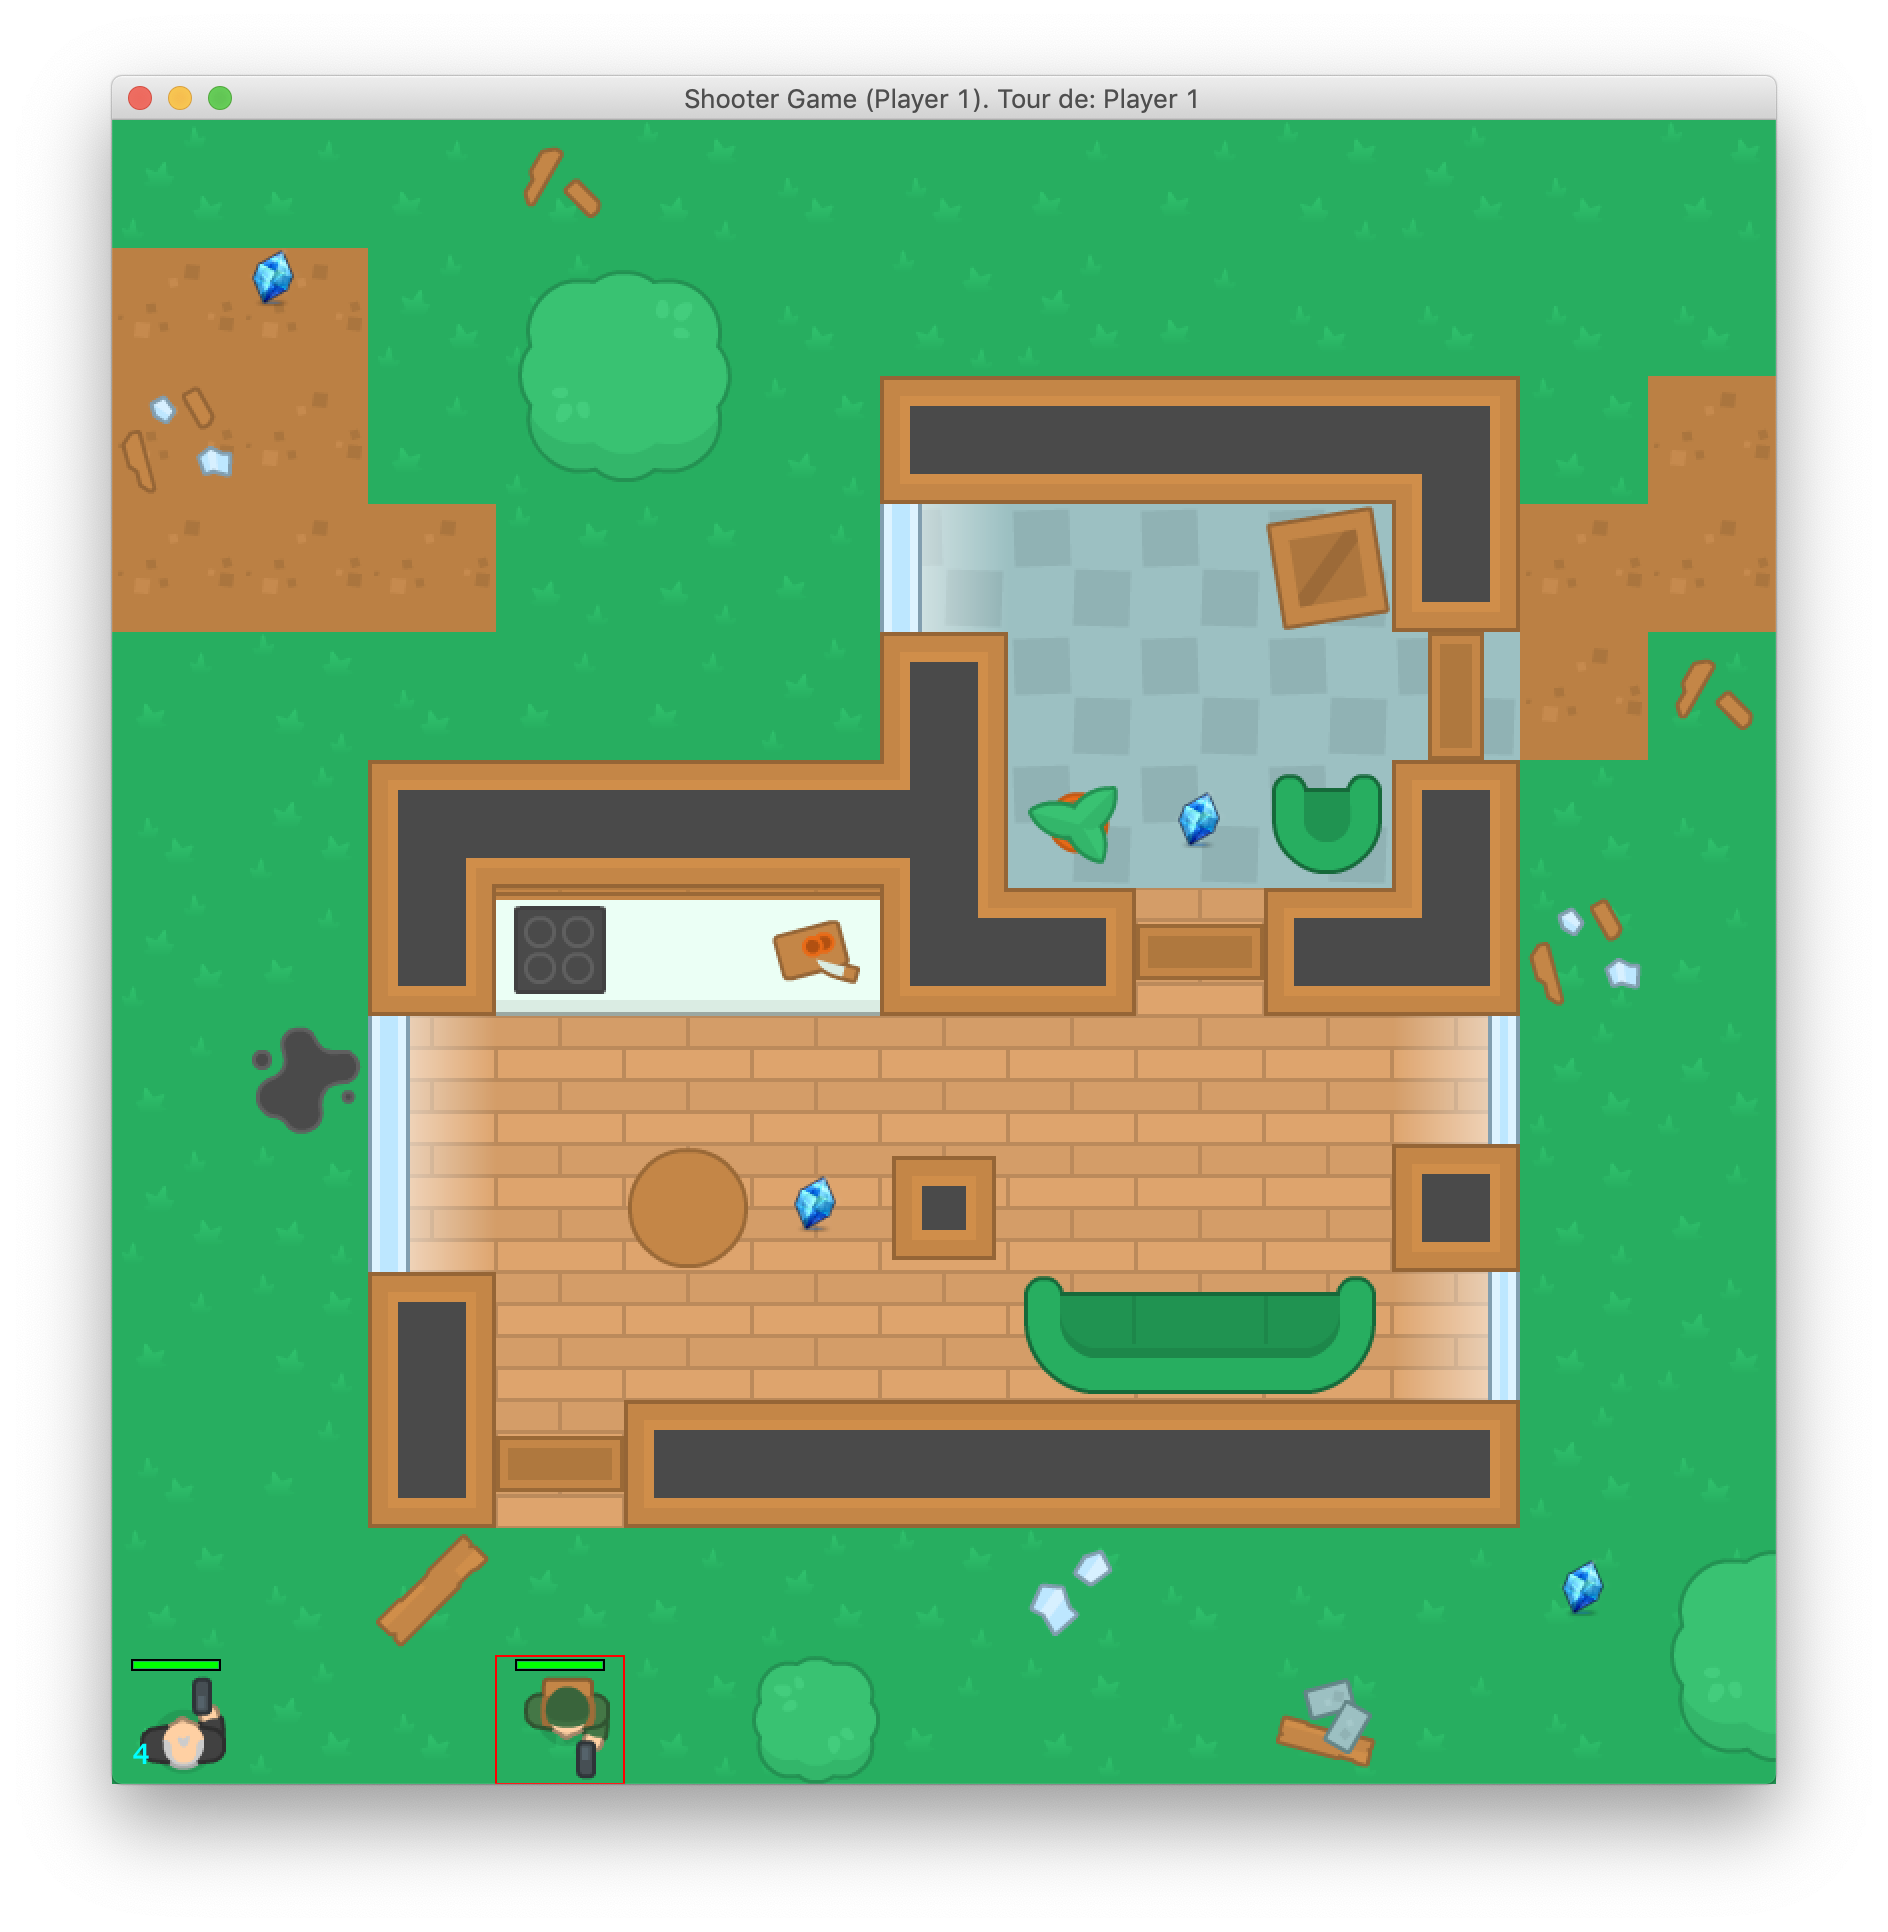
\includegraphics[scale=0.2]{images/interface.png}
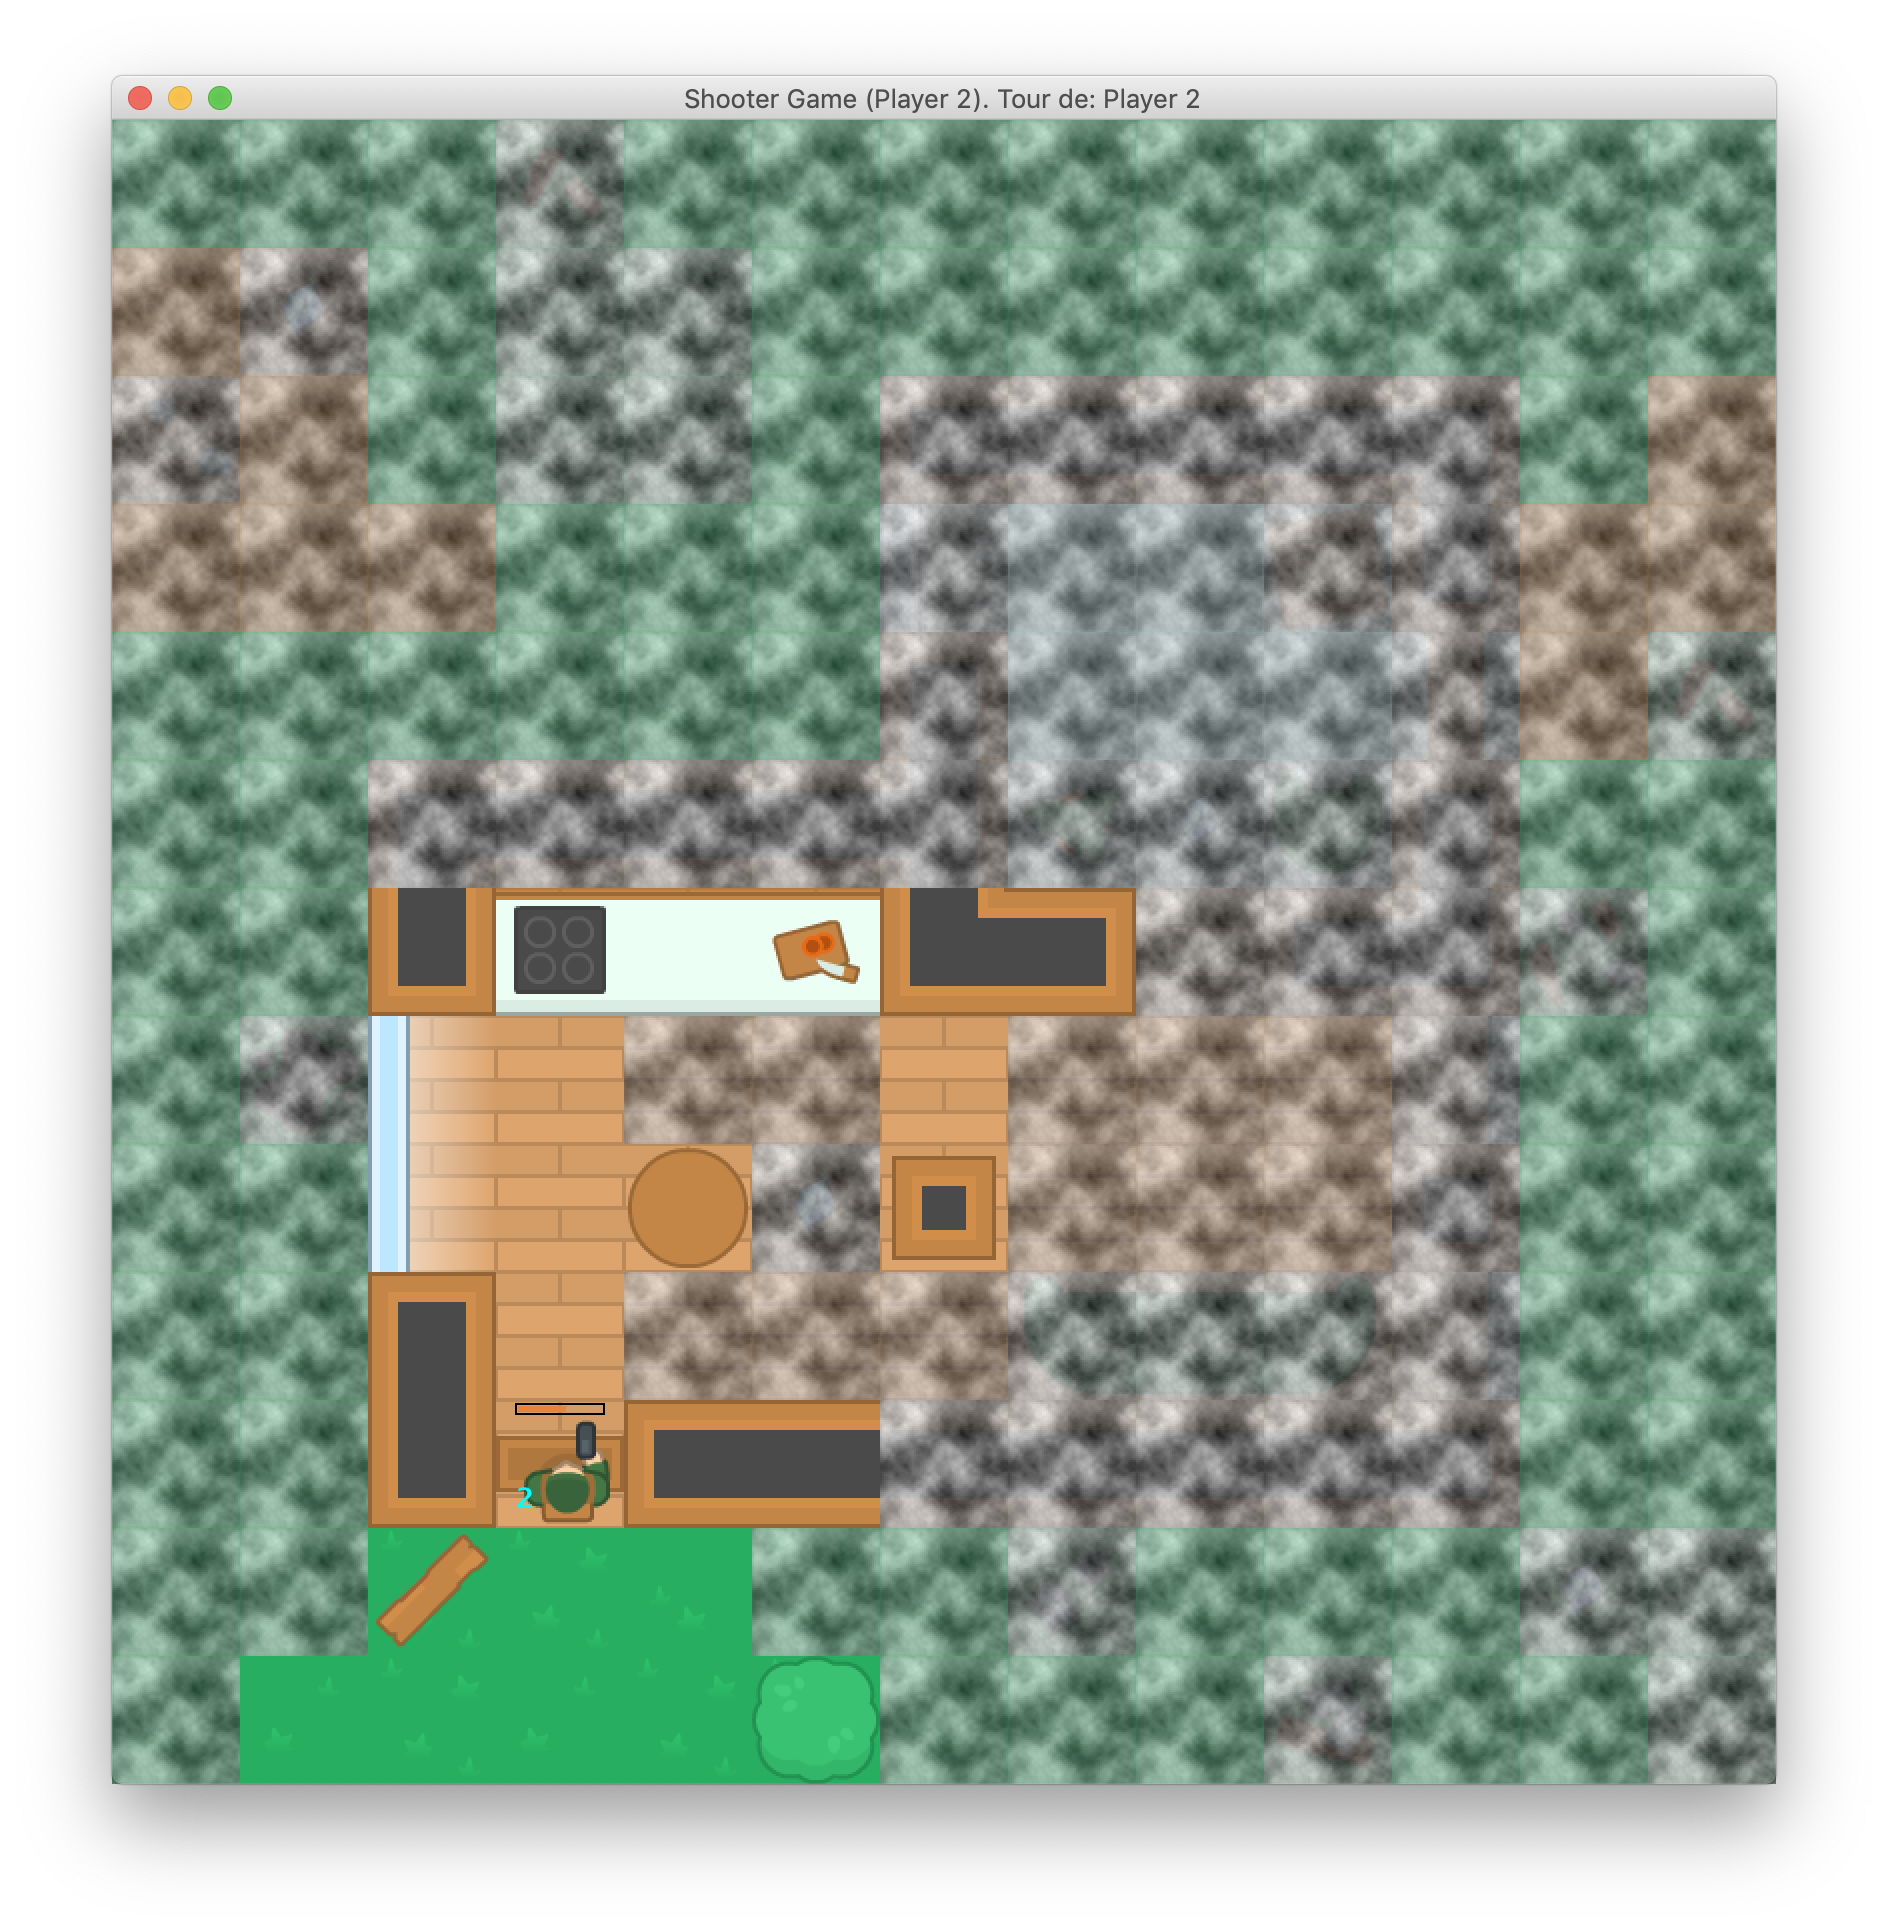
\includegraphics[scale=0.2]{images/interfaceBrume.png}
\caption{L'interface avec et sans brouillard}
\end{figure}
\subsubsection{Constructeur et principe de fonctionnement}
Lorsque la vue est créée, on renseigne pour le constructeur :
\begin{itemize}
\item Le model à écouter
\item Le joueur propriétaire de la vue
\item La liste des entités
\item la JFrame contenant la vue: l'observer
\end{itemize}
\subsubsection{Fonctionnement, affichage et actualisation.}
Lors de l’affichage, la vue parcourt la liste d'entités dans un ordre défini. Cet ordre représente notamment les couches (layers) contenues dans le fichier XML permettant de charger le niveau. L'ordre de cette liste est très important puisque l'on vient superposer les images les unes aux autres pour ajouter du détail, comme par exemple les fauteuils, tables etc.\\
Lorsque le model change, l'appel de la méthode \textit{stateChange()} provoque une actualisation de toutes les vues écoutant le model.
\subsubsection{Un élément optionnel : l’animation de tir}
Lorsqu'un joueur tir, une animation se déclenche permettant de visualiser le parcours de sa balle. Cette animation est réalisée par le biais d'un Thread actualisant deux valeurs x et y tant que la portée maximale n'a pas été atteinte. A chaque actualisation, on prévient la vue pour qu'elle puisse se repeindre. La classe permettant cette animation est la classe \textit{ThreadPlay}. 
\subsection{La classe GUI}
La classe GUI est la classe permettant de créer une fenêtre accueillant la vue d'un joueur.
\subsubsection{Constructeur et principe du fonctionnement}
Lors de sa création cette classe reçoit en argument:
\begin{itemize}
\item Le modèle
\item Le joueur à qui la vue devra appartenir
\end{itemize}
La vue est ensuite créée au sein du constructeur.
\subsubsection{La jouabilité}
L'application est jouable au clique et au clavier. En effet pour chaque action le joueur doit d'abord cliquer sur son personnage pour faire afficher un menu déroulant de ses actions possibles. Toutefois, si le joueur souhaite effectuer plusieurs déplacements à la suite.
\subsubsection{Entrées claviers}
Pour lire les entrées claviers, on doit dans un premier temps invoquer la méthode \textit{setFocusable(true)} puis la méthode \textit{requestFocus()}. Puis ajouter un keyListener a la fenêtre. 
\subsubsection{Entrées souris}
La majorité des actions se font grâce aux cliques. Pour cela, on ajoute un \textit{mouseListener} à la fenêtre. Ensuite on agis en conséquence lorsque l'on reçoit un clique.
\end{document}